%
The given equation can be rewritten as
\begin{align}\label{eq:solutions/41/4/eq:quadraticparabola}
    16x^2+24xy+9y^2+105x+110y+225 = 0
\end{align}
Comparing this to the standard equation,
%\vec{x}^T\vec{V}\vec{x}+2\vec{u}^T\vec{x}+f = 0
\begin{align}
    \vec{V} = \vec{V}^T = \myvec{16 & 12\\12 & 9}, \quad \vec{u} = \myvec{\frac{105}{2} \\ 55}, \quad f = 225 \label{eq:solutions/41/4/eq:Vufvals}
\end{align}
The characteristic equation of $\vec{V}$ is given as
\begin{align}
    \mydet{\lambda\vec{I}-\vec{V}} = 0\\
    \implies \mydet{\lambda-16 & -12 \\ -12 & \lambda-9} = 0\\
    \implies \lambda^2 -25\lambda = 0 \label{eq:solutions/41/4/eq:lambdaeq}
\end{align}
The eigenvalues are the roots of the equation \eqref{eq:solutions/41/4/eq:lambdaeq}, which are as follows :
\begin{align}
    \lambda_1 = 0, \quad \lambda_2 = 25 \label{eq:solutions/41/4/eq:eigenval}
\end{align}
The eigen vector $\vec{p}$ is defined as, 
\begin{align}
    \vec{V}\vec{p} &= \lambda\vec{p}\\
    \implies(\lambda\vec{I}-\vec{V})\vec{p}&=0
\end{align}
For $\lambda_1=0$
\begin{align}
    (\lambda_1\vec{I}-\vec{V}) = \myvec{-16 & -12\\-12 & -9}\xleftrightarrow[R_2\leftarrow R_2-3R_1]{R_1\leftarrow \frac{1}{4}R_1}\myvec{-4 & -3\\0 & 0}
\end{align}
\begin{align}
    \implies\vec{p_1}&=\frac{1}{5}\myvec{-3\\4}\label{eq:solutions/41/4/eq:p1val}
\end{align}
For $\lambda_2=25$
\begin{align}
    (\lambda_2\vec{I}-\vec{V}) = \myvec{9 & -12\\-12 & 16}\xleftrightarrow[R_2\leftarrow R_2+4R_1]{R_1\leftarrow \frac{1}{3}R_1}\myvec{3 & -4\\0 & 0}
\end{align}
\begin{align}
    \implies\vec{p_2}=\frac{1}{5}\myvec{4\\3}\label{eq:solutions/41/4/eq:p2val}
\end{align}
So, using Eigenvalue decomposition, $\vec{P}^T\vec{V}\vec{P}=\vec{D}$, where
\begin{align}
    \vec{P} = \frac{1}{5}\myvec{-3 & 4\\4 & 3}\\
    \vec{D} = \myvec{\lambda_1 & 0\\0 & \lambda_2} = \myvec{0 & 0\\ 0 & 25}
\end{align}
Then, for the parabola
\begin{align}
    \text{focal length} = \abs{\frac{2\eta}{\lambda_2}} \label{eq:solutions/41/4/eq:focallen}\\
    \eta = \vec{p}_1^T\vec{u} = \frac{25}{2}\label{eq:solutions/41/4/eq:etaval}\\
    \intertext{Substituting values from \eqref{eq:solutions/41/4/eq:etaval} and \eqref{eq:solutions/41/4/eq:eigenval} in \eqref{eq:solutions/41/4/eq:focallen}, we get}
    \text{focal length} = 1
\end{align}
The standard equation of the parabola is given by
\begin{align}
    \vec{y}^T\vec{D}\vec{y} = -2\eta\myvec{1 & 0}\vec{y}
\end{align}
And the vertex $\vec{c}$ is given by
\begin{align}
    \myvec{\vec{u}^T + \eta\vec{p}_1^T \\ \vec{V}}\vec{c} = \myvec{-f \\ \eta\vec{p}_1 - \vec{u}} \label{eq:solutions/41/4/eq:c}
\end{align}
Substituting values from \eqref{eq:solutions/41/4/eq:Vufvals},\eqref{eq:solutions/41/4/eq:etaval},\eqref{eq:solutions/41/4/eq:p1val} in \eqref{eq:solutions/41/4/eq:c},
\begin{align}
    \myvec{45 & 65\\16 & 12\\12 & 9}\vec{c} = \myvec{-225\\-60\\-45}
\end{align}
To find $\vec{c}$, performing row reduction on the augmented matrix as follows:
\begin{align}
    \myvec{45 & 65 & -225\\16 & 12 & -60\\12 & 9 & -45}\xleftrightarrow[R_1\leftarrow \frac{1}{45}R_1]{R_3\leftarrow R_3-\frac{3}{4}R_2}\myvec{1 & \frac{13}{9} & -5\\16 & 12 & -60\\0&0&0}\\
    \xleftrightarrow{R_2\leftarrow R_2-16R_1}\myvec{1 & \frac{13}{9} & -5\\0 & \frac{-100}{9} & 20\\0&0&0}\\\xleftrightarrow{R_2\leftarrow \frac{-9}{100}R_2}\myvec{1 & \frac{13}{9} & -5\\0 & 1 & \frac{-9}{5}\\0&0&0}\\\xleftrightarrow{R_1\leftarrow R_1-\frac{13}{9}R_2}\myvec{1 & 0 & \frac{-12}{5}\\0 & 1 & \frac{-9}{5}\\0&0&0}
\end{align}
Thus,
\begin{align}
    \vec{c} = \myvec{\frac{-12}{5}\\\frac{-9}{5}} = \myvec{-2.4 \\ -1.8}
\end{align}
\begin{figure}[h!]
    \centering
    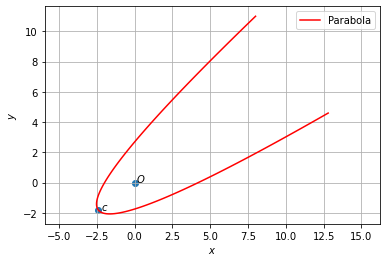
\includegraphics[width=\columnwidth]{./solutions/41/4/assignment5parabola.png}
    \caption{Parabola with vertex c}
    \label{eq:solutions/41/4/fig:fig1}
\end{figure}
